\subsubsection{CocktailAvenue}\label{subsubsec:CocktailAvenue}
\paragraph{Aufbau}\label{subsubsec:Aufbau_CocktailAvenue}\mbox{}\\

Die Maschine CocktailAvenue besteht aus einer Rückwand, an der die Getränkeflaschen mit dem Flaschenhals nach unten montiert werden können. In der Rückwand ist ein Touchpad verbaut, über welches die Cocktails ausgewählt werden können. Das Glas wird gefüllt, indem es auf einem Schlitten unter die Flaschen fährt und dann die Getränke eingefüllt werden. Der Schlitten wird mittels einem Zahnriemen hin und her gefahren. Das Auffüllen geschieht nicht mit Pumpen, sondern mit reiner Schwerkraft. Dosiert werden die Getränke mit Dosiergeräten, wie man sie aus den Bars kennt. Dabei wird eine Fixe Dosis (meist 2cl) hinaus gelassen. Die Dosiereinheit wird geöffnet, indem ein Hubzapfen aus der Halterung des Schlittens nach oben gefahren wird. Es gibt jedoch auch zwei Hahnen, aus denen Getränke hinausgelassen werden können. Vermutlich werden dort Pumpen eingesetzt.\cite{igus_automatisiertes_nodate}

\paragraph{Bedienung}\label{subsubsec:Bedienung_CocktailAvenue}\mbox{}\\

Die Bedienung geschieht über das Touchpad, welches in der Rückwand verbaut ist.\cite{igus_automatisiertes_nodate}

\paragraph{Technische Daten}\label{subsubsec:Technische_Daten_CocktailAvenue}\mbox{}\\

\begin{tabular}{@{}llp{0.6\textwidth}}
    Zeit für einen Cocktail: & : & Für die Zubereitung eines Cocktails braucht die Maschine gemäss einem Beispiel eines Youtube-Videos 25 Sekunden. \cite{cocktail_1_2017}\\
    \hline
    Anzahl verschiedene Cocktails: & : & Es wurden keine Angaben über die Anzahl verschiedene Cocktails gefunden. \\ 
    \hline
    Stromversorgung: & : & Der Cocktailmixer benötigt in jedem Fall einen Festanschluss an das Stromnetz.\cite{igus_automatisiertes_nodate} \\
\end{tabular}

\newpage

\paragraph{Reinigung}\label{subsubsec:Reinigung_CocktailAvenue}\mbox{}\\

Die Reinigung gestaltet sich bei der CocktailAvenue ziemlich einfach. Da es keine Pumpen und Schläuche gibt, entfällt ein sehr grosser Teil. Einzig die Dosiergeräte müssen zwischendurch demontiert und sauber gemacht werden. Auch der mechanische Aufbau der Schiene unterhalb der Getränke wurde so konzipiert, dass eine Reinigung sehr einfach ist und eventuelle Verunreinigungen den Betrieb nicht beeinflussen.\cite{igus_automatisiertes_nodate}

\paragraph{Sonstiges}\label{subsubsec:Sonstiges_CocktailAvenue}\mbox{}\\

Die Antriebstechnik geschieht mit einer Zahnriemenachse. Sie besteht aus einem Aluprofil. Die Achse muss nicht geschmiert werden, was demnach bei Anwendungen mit hohen Hygieneanforderungen sehr vorteilhaft ist. Ebenso wird so ein wartungsfreier Betrieb gewährleistet. Der Antrieb wird mit einem Schrittmotor realisiert, was eine vibrationslose Bewegung garantiert. Damit die Kabel bei Bewegungen sauber geführt und nicht geknickt werden, wird eine Kabelkette verwendet. Zukünftig plant der Hersteller eine Erweiterung der modular aufgebauten Baureihe. Mittlerweile gibt es auch eine Version, bei der die Antriebsachse im Gehäuse verbaut ist. Die exakte Positionierung des Schlittens unter den Flaschen muss nicht sehr genau sein, da die Achse nach jeder Zubereitung wieder den Ausgangs- und Referenzpunkt anfährt. \cite{igus_automatisiertes_nodate}

\begin{figure}[h]
	\centering
	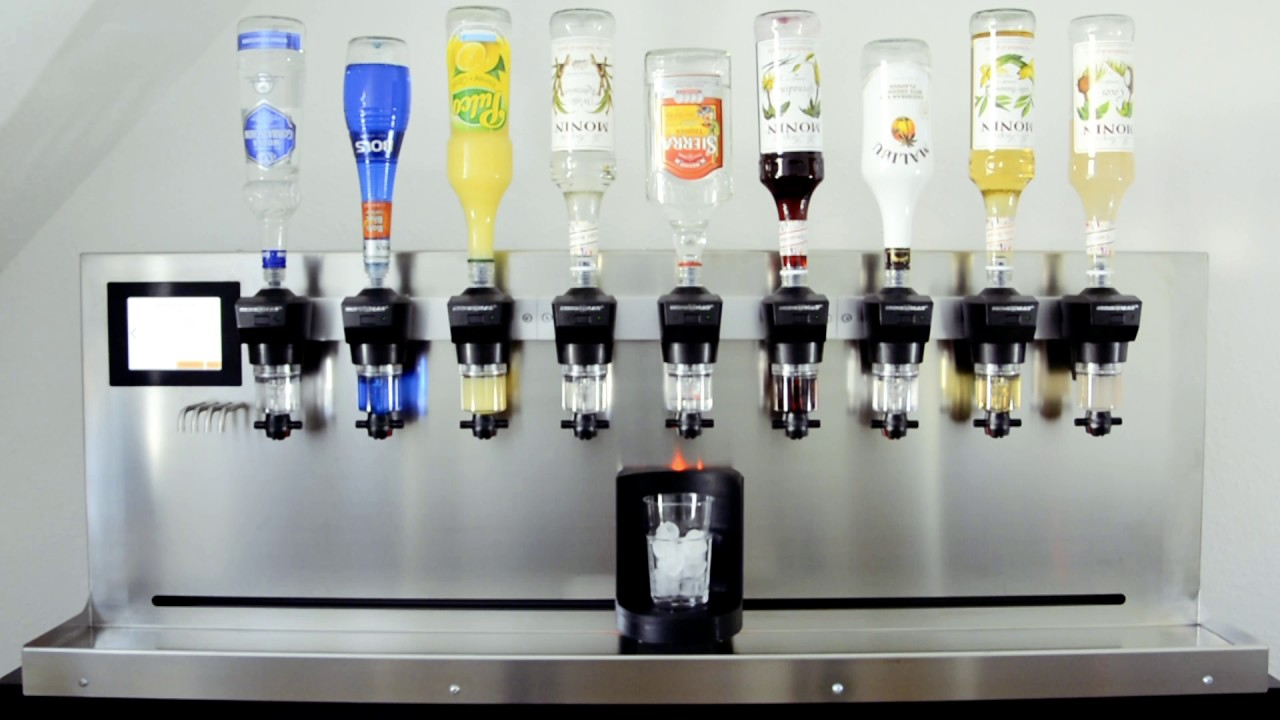
\includegraphics[width=0.5\textwidth]{graphics/CocktailAvenue.jpg}
	\caption{CocktailAvenue \cite{igus_automatisiertes_nodate}}
	\label{fig:CocktailAvenue_Cocktailmaschine}
\end{figure}